\subsection{The multi-VoF methodology and the no-coalescence algorithm}
% Objectives 
% \begin{itemize}
%     \item Presents the bibliography. 
%     \item Introduce mani's algorithm
%     \item explain step by step the algorithm
%     \item Color map theorm for 3D 
% \end{itemize}


The key feature of numerical simulations is the use of a whole new algorithm which prevent numerical coalesce of droplets to occur.
First, the reader can find the described source code at \href{https://basilisk.fr/sandbox/fintzin/no-coalesce.h}{no-coalesce.h}. 
In the following we describe the global ideas and principles, then we dive into a step by step explanation of the algorithm. 
But first some worlds on the already existing algorithm is in order.

In previous studies several methods have been used to avoid coalescence. 
The first one is to increase artificially the surface tension coefficient locally such as it is done in the recent study of \citet{hidman2023assessing}.
Although, this method seems very efficient, it is unclear if physical behavior of the droplets' interaction dynamic is well represented because of the added artificial forces. 
In  \citet{balcazar2015multiple} they developed a multiple marker level-set method to prevent coalescence. 
In the recent study of \citet{zhang2021direct} they  used one VoF tracer per bubble in his simulation which prevent coalescence and allows tracking bubbles independently. 
However, this approach is quite expensive as it requires solving a transport equation for each VoF tracer, meaning each drop. 
Instead, we adopt the methodology of \citet{karnakov2022computing} which consider a number of VoF tracers not correlated with the number of droplets, such that several non-touching droplets are the same VoF tracer fields.
This last methodology makes the simulation a lot less expensive since it require only a finite number of VoF tracers for an arbitrary umber of non coalescing droplets.  
Therefore, in the following we adopt this methodology within the \texttt{Basilisk} code. 

The challenge here is to color every adjacent droplets with a VoF tracer, so that they do not numerically merges, but with the least number of VoF tracer as possible. 
This recall the famous \textit{Four color map theorem} \citep{kempe1879colours} which basically state that : 
\enquote{every map can be color using only four colors, so that two neighboring region are different colors}. 
In our case, it means that for any 2D configuration only four VoF tracer might be used to avoid coalesce\footnote{Actually on a bi-periodic domain 7 color is needed since the periodic boundary condition makes the domain having torus-like topology, in which case 7 color is required.  }. 
Which is far less than one tracer for each droplet. 
In case of maps the optimal coloring is applied to a static graph. 
In our case droplets may move around over time changing the graph over time. 
Our problem is thus a time-varying graph coloring problem where the optimal coloring must be recomputed at each time step.
Additionally, even if a solution exist in 2D configuration, these problems are theoretically expensive to solve (NP-complete) and even more complexe to solve at each time step.  
In the three-dimensional space it is easy to find counter examples to the \textit{Four color map theorem}. 
% One of them is shown \ref{fig:colors}, where five 3 dimensional objects all touch each other so that five color is needed. 
For example, an infinite number of rectangular blocks in 3D spaces can all touch each other requiring an infinite number of colors to differentiate adjacent blocks\citep{magnant2011coloring}. 
% \begin{figure}
%     \centering
%     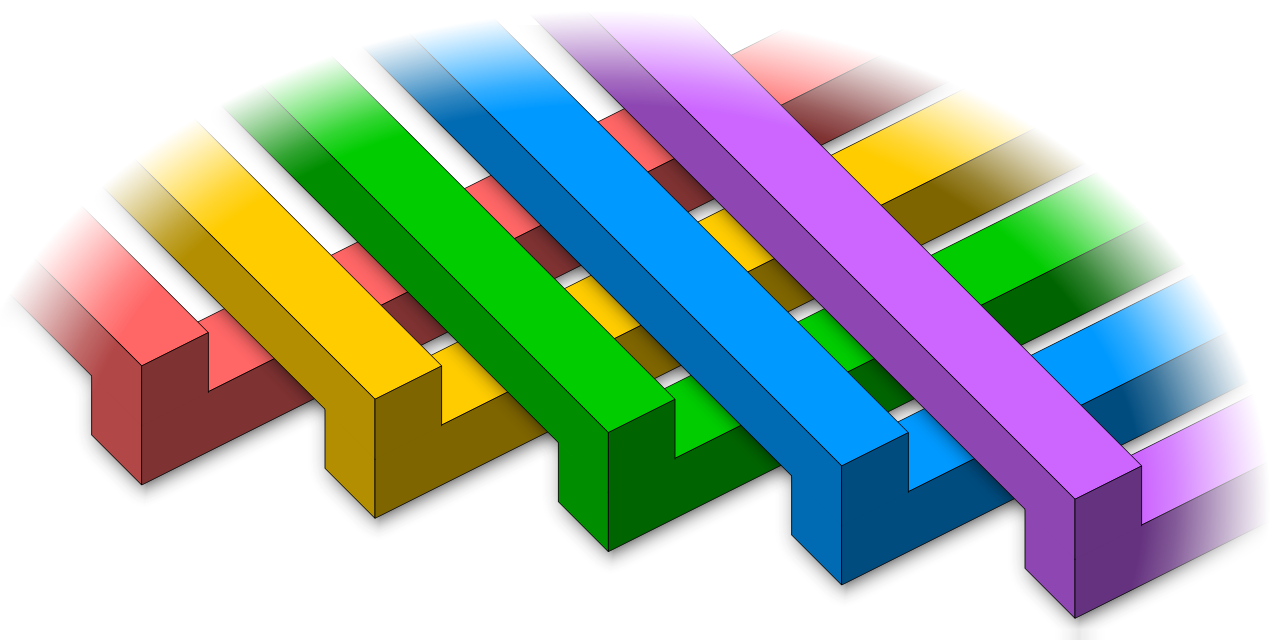
\includegraphics[width=0.5\textwidth]{image/more_than_four.png}
%     \caption{
%     Proof of the non validity of the \textit{Four color map theorem} in three-dimensional spaces. 
%     3 dimensional pictures of five regions all touching each other. 
%     Clearly, in this case 5 color is required. 
%     }
%     \label{fig:colors}
% \end{figure}
From the knowledge of the author no such problem has been solved for 3D spheres, however we believe that there is no way to find an optimal coloring configuration for spheres in the 3 dimensional space based on topological arguments. 
Nevertheless, it is reasonable to believe that the number of tracer required to avoid coalescence is fewer than the number of droplets.
Consequently, since we can not determine the optimal coloring configuration based on theoretical ground, we choose to assign VoF tracers to each droplet following the strategy detailed below.

The development of the \texttt{no-coalesce.h} algorithm within the basilisk framework was initiated in the PhD. thesis of \citet{mani2021numerical}.
They developed an algorithm to prevents the adjacent droplets to have similar VoF tracers, using the least VoF tracer as possible by allowing different drops to be included within the same VoF tracer.
We now present the methodology of this algorithm extended to 3 dimensional flows.
As the methodology remain essentially the same for 2D and 3D we redirect the reader to \citet{mani2021numerical} PhD. for a precise description of the algorithm. 
Again, the reader can directly look at the documented source code available in the basilisk wiki page : \href{http://basilisk.fr/sandbox/fintzin/Rising-Suspenion/no-coalescence.h}{no-coalescence.h}.
In the following we summarize the workflow of this algorithm. 

But, before we need to introduce a key feature used in these simulations, the \href{http://basilisk.fr/src/tag.h}{tag.h} algorithm. 
It is an adaptation of the \textit{scanline fill algorithm} in optimized by the use of with the multigrid solver. 
The goal of this algorithm is to assign a different scalars values to each cell's belonging to different region such as a droplets. 
For example on \ref{fig:images} (left) we can see that the two blue region, are assigned with 2 different tag value. 
Consequently, through the use of this algorithm we can identify the different droplets present in a single VoF fields. 
To track the bubbles independently while several of them are contained in the same VoF tracer we also make use of this algorithm.   
Indeed, it is simple to obtain a droplet property, such as its center of mass position or velocity, by carrying numerical integration on the VoF fields keeping only the cells having a specific tag value which correspond to a given drop.  


We define the $i^\text{th}$ VoF tracer as $C_i$ for $i =0,\ldots,N(t)$, where $N(t)$ is the total number of VoF tracer used in a simulation at time $t$.
The color function introduced in \ref{eq:dt_C} can be written as, $\sum_i^{N(t)} C_i$. 
Notice that $N(t)$ is time dependent since the number of VoF tracer might increase along the simulation time as the droplets get in contact. 
Indeed, the adjacent droplets at a given time $t$ must have different VoF tracer to prevent coalescence. 
The simplified workflow of the algorithm follows these three steps : 
\begin{enumerate}
    \item[Step 1.] We first check if within a VoF tracer $C_i$, the droplets are possibly too close to each other. 
    The distance criterion is defined such that we search for cells where $C_i > 1$, with a requirement that they are within a maximum separation of five cells, and the intermediate cells between them have $C_i = 0$.
    % In which case, two different topology might be present because the center cell is empty, and too close because they are 5 cells apart.
    A scheme of the criterion is given in \ref{fig:criterion}.  
    At this stage we identified within a single VoF tracer if surfaces might be too close to each other such as in \ref{fig:criterion} (right) or \ref{fig:criterion} (left).
    \item[Step 2.] 
    If (Step 1.) is true we must identify the different topologies present in the VoF tracer $C_i$. 
    Indeed, (Step 1.) can be true for a region touching itself as depicted  \ref{fig:diagram} (right), in which case we do not want to interfere. 
    % Therefore, we must be able to identify groups in the VoF fields which define the different topologies. 
    In \ref{fig:criterion} (left) we observe that each blue drops posses two different tags values, namely $1$ and $2$, witnessing of their topological independence.
    In this case we are sure that two droplets are nearly colliding.  
    Note that two adjacent drops belonging to two different VoF tracer can possess the same tag values as VoF tracers are independent. 
    \item[Step 3.] Then we re-use the distance criterion depicted \ref{fig:criterion} by requiring in addition that the cells must belong to two different tags groups. 
    In which case we are sure that we are in presence of two cells belonging to the same VoF tracer but not to the same drops that are nearly touching.
    At this stage the situation \ref{fig:criterion}(left) would be true but the situation \ref{fig:criterion}(right) would be false. 
    \item[Step 4.] Lastly, we assign a new VoF tracer for each droplet/tags that are too close to another. 
    If the droplet is not adjacent to another tracer, let's say the VoF tracer $C_j$ with $j \in [0,N]$, we assign to the droplet the tracer $C_j$ or any other that isn't adjacent. 
    Clearly, in \ref{fig:criterion}(right) the droplet on the right is adjacent to the VoF tracer $C_j$ in which case we must find an other VoF tracer $C_e$ with $e \neq i,j$. 
    If the droplet is already adjacent to every tracer $C_j$ for $j = 1,2\ldots N$, we create a new VoF tracer, named $C_j$  with $j = N+1$ and assign it to the droplet. 
\end{enumerate}
\begin{figure}
    \centering
    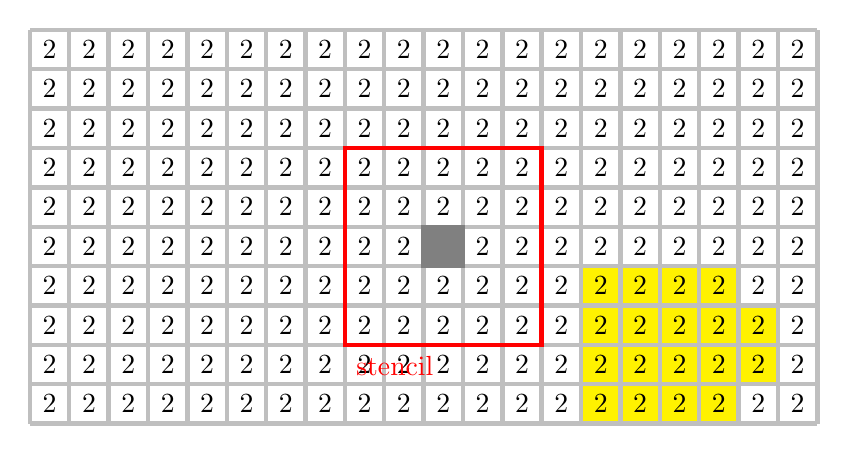
\begin{tikzpicture}[scale=0.5,ultra thick]
        % Define grid dimensions
        \def\nRows{10}
        \def\nCols{20}
        \pgfmathsetmacro\nRowsm{\nRows-1}
        \pgfmathsetmacro\nColsm{\nCols-1}

        \foreach \row in {0,...,\nRowsm} {
            \foreach \col in {0,...,\nColsm} {
                \pgfmathsetmacro\distance{veclen(\col-4.356, \row-2.65)};
                \pgfmathparse{\distance < 4 ? "blue" : "white"}
                \edef\colour{\pgfmathresult};
                \ifthenelse{\equal{\colour}{blue}}{                    
                    \fill[\colour!60!white] (\col, \row) rectangle ++(1,1);
                    \node (num) at (\col +0.5,\row+0.5){1};
                }
            }
        }

        \foreach \row in {0,...,\nRowsm} {
            \foreach \col in {0,...,\nColsm} {
                \pgfmathsetmacro\distance{veclen(\col-15, \row-6.2)};
                \pgfmathparse{\distance < 3.5 ? "blue" :"white"}
                \edef\colour{\pgfmathresult};
                \ifthenelse{\equal{\colour}{blue}}{
                    \fill[\colour!60!white] (\col, \row) rectangle ++(1,1);
                \node (num) at (\col +0.5,\row+0.5){2};
                }
            }
        }

        \foreach \row in {0,...,\nRowsm} {
            \foreach \col in {0,...,\nColsm} {
                \pgfmathsetmacro\distance{veclen(\col-15.62, \row-1.5)};
                \pgfmathparse{\distance < 2.5 ? "yellow" :"white"}
                \edef\colour{\pgfmathresult};
                \ifthenelse{\equal{\colour}{yellow}}{
                    \fill[\colour] (\col, \row) rectangle ++(1,1);
                    \node (num) at (\col +0.5,\row+0.5){2};
                }
            }
        }
        % Define grid size
        \pgfmathsetmacro\gridSize{1}
        
        \foreach \row in {0,...,\nRows} {
            \draw [gray!50] (0,\row*\gridSize) -- (\nCols*\gridSize,\row*\gridSize);
        }
        % Draw vertical grid lines
        \foreach \col in {0,...,\nCols} {
            \draw [gray!50] (\col*\gridSize,0) -- (\col*\gridSize,\nRows*\gridSize);
        }
        % Draw drop shape
        \draw[red] (8,2)node[below right]{stencil} rectangle +(5,5); % Draw the rectangular base
        \filldraw[gray] (10,4) rectangle +(1,1);
    \end{tikzpicture}    
    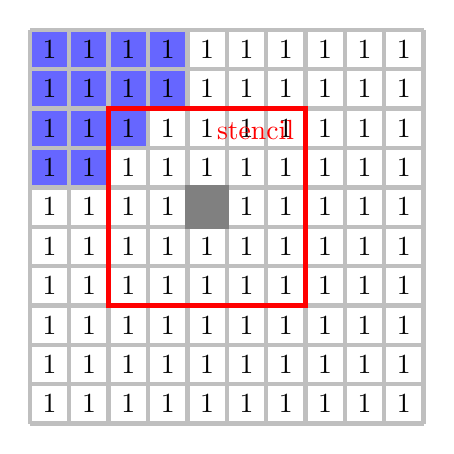
\begin{tikzpicture}[scale=0.5,ultra thick]
        % Define grid dimensions
        \def\nRows{10}
        \def\nCols{10}
        \pgfmathsetmacro\nRowsm{\nRows-1}
        \pgfmathsetmacro\nColsm{\nCols-1}

        \foreach \row in {0,...,\nRowsm} {
            \foreach \col in {0,...,\nColsm} {
                \pgfmathsetmacro\distance{veclen(\col, \row-2)};
                \pgfmathparse{\distance < 3.5 ? "blue" :"white"}
                \edef\colour{\pgfmathresult};
                \ifthenelse{\equal{\colour}{blue}}{
                    \fill[\colour!60!white] (\col, \row) rectangle ++(1,1);
                \node (num) at (\col +0.5,\row+0.5){1};
                }
            }
        }

        \foreach \row in {0,...,\nRowsm} {
            \foreach \col in {0,...,\nColsm} {
                \pgfmathsetmacro\distance{veclen(\col-7, \row-2)};
                \pgfmathparse{\distance < 3.5 ? "blue" :"white"}
                \edef\colour{\pgfmathresult};
                \ifthenelse{\equal{\colour}{blue}}{
                    \fill[\colour!60!white] (\col, \row) rectangle ++(1,1);
                    \node (num) at (\col +0.5,\row+0.5){1};
                }
            }
        }
        \foreach \row in {0,...,\nRowsm} {
            \foreach \col in {0,...,\nColsm} {
                \pgfmathsetmacro\distance{veclen(\col-5, \row)};
                \pgfmathparse{\distance < 3.5 ? "blue" :"white"}
                \edef\colour{\pgfmathresult};
                \ifthenelse{\equal{\colour}{blue}}{
                    \fill[\colour!60!white] (\col, \row) rectangle ++(1,1);
                    \node (num) at (\col +0.5,\row+0.5){1};
                }
            }
        }
        \foreach \row in {0,...,\nRowsm} {
            \foreach \col in {0,...,\nColsm} {
                \pgfmathsetmacro\distance{veclen(\col, \row-9)};
                \pgfmathparse{\distance < 3.5 ? "blue" :"white"}
                \edef\colour{\pgfmathresult};
                \ifthenelse{\equal{\colour}{blue}}{
                    \fill[\colour!60!white] (\col, \row) rectangle ++(1,1);
                    \node (num) at (\col +0.5,\row+0.5){1};
                }
            }
        }
        % Define grid size
        \pgfmathsetmacro\gridSize{1}
        
        \foreach \row in {0,...,\nRows} {
            \draw [gray!50] (0,\row*\gridSize) -- (\nCols*\gridSize,\row*\gridSize);
        }
        % Draw vertical grid lines
        \foreach \col in {0,...,\nCols} {
            \draw [gray!50] (\col*\gridSize,0) -- (\col*\gridSize,\nRows*\gridSize);
        }
        % Draw drop shape
        \draw[red] (2,3) rectangle +(5,5)node[below left]{stencil}; % Draw the rectangular base
        \filldraw[gray] (4,5) rectangle +(1,1);
    \end{tikzpicture}    
    \caption{Scheme of the \textit{near contact} criterion adopted in the \texttt{no-coalesce.h} algorithm. 
    The background grid represents the cells within the numerical domain. 
    The dark blue area represents the cells where $C_i > 0$.
    The yellow area represents the cells where the VoF tracer $C_j > 0$ for $j\neq i$. 
    The numbers represent the value of the $Tag$ scalar fields within each VoF tracer.
    Two droplets can possess the same tag as long as they are not in the same VoF tracer. 
    The 5 by 5 red rectangle represent the stencil zone which iterate over all cells where the center of the stencil (gray square) respect $C_i = 0$. 
    (left)
    Clearly, in this situation we identified two droplets in contact since we observe two opposite cells in the stencil with $C_i > 0$ and $C_i=0$ at the center.
    And, the mentioned cells belong to two different topologies so that (\textit{Step 3}) is also validated.  
    (right) In this situation we identified a near contact with since we observe two opposite cells in the stencil with $C_i > 0$ and $C_i=0$ at the center, however in this case we do not complete the second criterion of (\textit{Step 3}) which require two different topologies. 
    }
    \label{fig:criterion}
\end{figure}

These four steps ares executed at each simulation time step for each VoF tracer : $C_i$. 
Having $N(t)$ VoF tracer require some modifications to the previously mentioned governing equations. 
Especially, instead of solving \ref{eq:dt_C}  we solve $N(t)$ transport equation for each VoF tracer and we compute the surface tension force as the sum of the contribution from each VoF tracer independently.
Therefore, we solve these equations, 
\begin{align*}
    \pddt C_i + \textbf{u}\cdot\grad C_i = 0.
    \ \  \ \ \forall i \in [0,N(t)]\\
    \textbf{f}_\gamma 
    = \sum_{i=0}^{N(t)} \gamma \kappa_i \grad C_i
\end{align*}
where $\kappa_i$ is the approximate curvature of a single $C_i$ which is computed with height function the classic method employed for a single VoF-tracer. 
Regarding the performances of the algorithm \ref{fig:diagram} (left) shows a Snapshot of a DNS at an arbitrary time $t^* = 100$ within which we can observe the droplets' interface colored by their VoF tracer. 
It is clear that in this simulation no more than 3 color was needed to avoid coalesce, at that time.
\ref{fig:diagram} (right) display the number of VoF $N(t)$ in terms of the dimensionless simulation time and volume fraction $\phi$. 
We observe that for an entire simulation no more than 3 VoF tracer were used for $\phi = 0.01$ up to $7$ for the denser case $\phi = 0.2$. 
Although our algorithm is far from being theoretically optimal, we believe that it brings sufficient efficiency for our need. 
\begin{figure}[h!]
    \centering
    % \begin{tikzpicture}[scale=0.1,
    %     node distance = 4mm and 6mm,
    %   start chain = going below,
    %   base/.style = {draw, thick, fill=gray!10, align=center, 
    %                  inner xsep=2mm, inner ysep=2mm},
    %   rect/.style = {base},
    %   elli/.style = {ellipse, base},
    %   circ/.style = {circle, fill=graye!10, minimum size=12pt},
    %   diam/.style = {diamond, base, aspect=1.5},
    %   line/.style = {draw, rounded corners, -Stealth, semithick},
    % ]
    % % Place nodes
    % \begin{scope}[nodes = {on chain, join=by line}]
    % \node [rect, rounded corners=10pt] (step1) {start};
    % \node [rect] (step15) {(1) \texttt{bubbles\_are\_close}($C_i$)};
    % \node [rect] (step2) {(2) Apply tag function \\ on VoF field $C_i$};
    % \node [base] (step3) {(3) Check for any cells adjacent drops \\ that have the same $C_i$};
    % \node [rect] (step5) {(4) Change drops VoF tracers for all\\ adjacent drops.};
    % \node [diam] (step7) {$i < N(t)$};
    % \node [rect, rounded corners=10pt] (step8) {stop};
    % \end{scope}
    % \node [rect, left=of step3] (step9) {$i = i+1$};
    % Draw edges
    % \path[line] (step7) -| (step9);
    % \path[line] (step9) |- (step15);
    % %
    % \path       (step7) -- node [right,near start]{False}    (step8);
    % \path       (step15) -| (step7); % node [right,near start]{False}    (step7);
    % \node [right=of step5] {lala};
    % \end{tikzpicture}
    \begin{tikzpicture}
    \node (img) at (0,0) {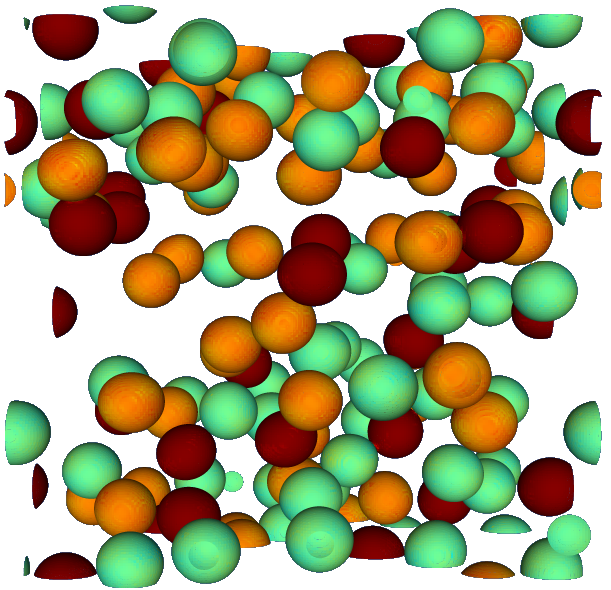
\includegraphics[width = 0.4\textwidth]{image/VoF2.png}};
    \node (img) at (0.4\textwidth,-0.01\textwidth) {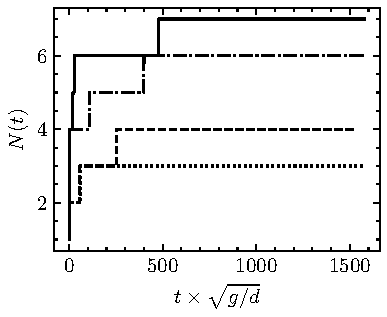
\includegraphics[width = 0.35\textwidth]{image/HOMOGENEOUS_NEW/CA/NVoF_vs_t_Ga_50_l_1.pdf}};
    \end{tikzpicture}
    \caption{
    (left) Snapshot of a DNS with $\phi = 0.05$, $\lambda = 1$, $Ga = 50$ with the interface of the droplets colored by the index of the VoF tracer.
    (right) Number of VoF tracer versus dimensionless time  at $t^*$.
    Four different volume fractions are displayed : (dotted line) $\phi = 0.01$, (dashed line) $\phi = 0.05$ (dash dotted line) $\phi = 0.1$ (solid line) $\phi = 0.2$ at $Ga = 50$ and $\lambda = 1$. 
    }
    \label{fig:diagram}
\end{figure}

\tb{mettre le cout de calcul associé au VoF N(t) : dtrace=-2}




At this stage one might wounder : is the physics of droplets interaction well captured due to the use of the multi VoF method ?
Indeed, with a grid definition of $\Delta = d/30$ the film between the drops is not accurately solved, so how accurate is are interaction between droplets ?
Answer is  provided in \ref{ap:validation} (\textit{Case 2.}) where we validate our multi-VoF method to \citet{mohamed2003drop} experiments.
In \citet{mohamed2003drop} they study experimentally the impact of a single drop on a flat interface, while recording the position of the interfaces. 
It is found that the mult-VoF method capture well the dynamic of interfaces with a poor description of the liquid film between these interfaces ($\Delta = d/30$). 
However,  \citet{mohamed2003drop} experiment were carried at $Bo = 6$ which is significantly higher than our range of \textit{Bond} number. 
It is possible than at lower \textit{Bond} number we obtain poorer agreements with reality due to a different flow behavior present in the film inducing more viscous dissipation.
The viscous dissipation might require more grid point in the film. 
Nevertheless, we argue that the mesh definition independence study conducted in \ref{ap:validation} substantiates the accuracy of the DNS since dynamic of interaction does converge for a grid definition of $\Delta = d/30$. 
Overall, we used an optimized multi-VoF method which allows us to compute massive DNS with a maximun of $7$ VoF tracers for dense emulsion.
 





